\documentclass[10pt,a4paper]{article}

\usepackage[margin=16mm,headheight=14pt,footskip=12mm]{geometry}
\usepackage{fontspec}
\usepackage{amsmath,amssymb,mathtools}
\usepackage{microtype}
\usepackage{xcolor}
\usepackage{tikz}
\usetikzlibrary{arrows.meta,positioning,calc,fit,matrix}
\usepackage[most]{tcolorbox}
\usepackage{enumitem}
\usepackage{titlesec}
\usepackage{fancyhdr}
\usepackage{ragged2e}

\IfFileExists{/usr/share/fonts/opentype/urw-base35/NimbusSans-Regular.otf}{
  \setmainfont[
    Path=/usr/share/fonts/opentype/urw-base35/,
    UprightFont=NimbusSans-Regular.otf,
    BoldFont=NimbusSans-Bold.otf,
    ItalicFont=NimbusSans-Italic.otf,
    BoldItalicFont=NimbusSans-BoldItalic.otf
  ]{Nimbus Sans}
  \setsansfont[
    Path=/usr/share/fonts/opentype/urw-base35/,
    UprightFont=NimbusSans-Regular.otf,
    BoldFont=NimbusSans-Bold.otf,
    ItalicFont=NimbusSans-Italic.otf,
    BoldItalicFont=NimbusSans-BoldItalic.otf
  ]{Nimbus Sans}
}{
  \setmainfont{DejaVu Sans}
  \setsansfont{DejaVu Sans}
}
\setmonofont{DejaVu Sans Mono}

\definecolor{navy}{HTML}{102E50}
\definecolor{blue}{HTML}{2F75B5}
\definecolor{bluefill}{HTML}{EAF3FB}
\definecolor{slatefill}{HTML}{F3F6F9}
\definecolor{slate}{HTML}{607080}
\definecolor{red}{HTML}{9E2525}
\definecolor{redfill}{HTML}{FDEDED}
\definecolor{green}{HTML}{246B42}
\definecolor{greenfill}{HTML}{EAF7EF}
\definecolor{orange}{HTML}{9B5B00}
\definecolor{orangefill}{HTML}{FFF4E3}
\definecolor{rulegray}{HTML}{CBD5DF}

\pagestyle{fancy}
\fancyhf{}
\fancyhead[R]{\sffamily\bfseries\footnotesize\color{slate} LIGERO TECHNICAL NOTE}
\fancyfoot[C]{\sffamily\footnotesize\color{slate} Random projection in routed Ligero}
\renewcommand{\headrulewidth}{0pt}

\titleformat{\section}{\sffamily\bfseries\Large\color{blue}}{}{0pt}{}
\titlespacing*{\section}{0pt}{5pt}{5pt}
\setlength{\parindent}{0pt}
\setlength{\parskip}{3pt}
\setlist[enumerate]{leftmargin=7mm,itemsep=2pt,topsep=2pt}

\newtcolorbox{ideabox}{
  colback=bluefill,colframe=rulegray,boxrule=.6pt,arc=0pt,
  left=3mm,right=3mm,top=2.5mm,bottom=2.5mm
}
\newtcolorbox{resultbox}{
  colback=greenfill,colframe=green!45,boxrule=.6pt,arc=0pt,
  left=3mm,right=3mm,top=2.5mm,bottom=2.5mm
}

\tikzset{
  >={Latex[length=2mm]},
  flow/.style={->,draw=slate,line width=.65pt},
  dashedflow/.style={->,draw=slate!60,dashed,line width=.65pt},
  base/.style={draw=blue!55,fill=bluefill,rounded corners=2mm,minimum height=9mm,
               align=center,font=\sffamily\small,inner xsep=3mm},
  neutral/.style={draw=slate!45,fill=slatefill,rounded corners=2mm,minimum height=9mm,
                  align=center,font=\sffamily\small,inner xsep=3mm},
  active/.style={draw=red!45,fill=redfill,rounded corners=2mm,minimum height=9mm,
                 align=center,font=\sffamily\small,inner xsep=3mm},
  good/.style={draw=green!45,fill=greenfill,rounded corners=2mm,minimum height=9mm,
               align=center,font=\sffamily\small,inner xsep=3mm},
  router/.style={draw=orange!55,fill=orangefill,rounded corners=2mm,minimum height=9mm,
                 align=center,font=\sffamily\small,inner xsep=3mm},
  labeltext/.style={font=\sffamily\scriptsize,text=slate,align=center},
}

\begin{document}

{\sffamily\bfseries\fontsize{23}{27}\selectfont\color{navy}
Random Projection in Routed Ligero}\par
{\sffamily\itshape\color{slate}
Why it is needed, how it compresses the witness, and a complete numerical example.}

\begin{ideabox}
\textbf{\color{navy}Core idea.} Projection speeds up the proof by replacing a huge witness of
individual scalar multiplications with one randomized fingerprint check.
\end{ideabox}

\section*{1. Why the witness becomes too large}

{\sffamily\bfseries\color{navy}A. Three experts: only the selected route gets an activation trace}

\begin{center}
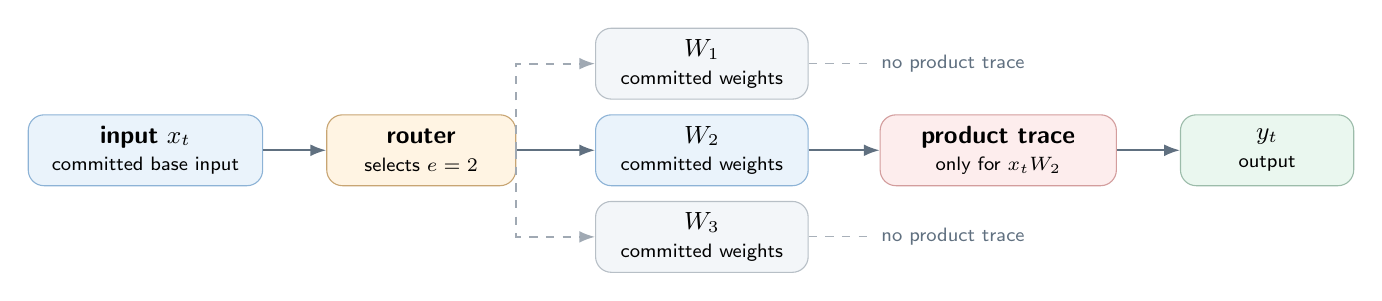
\begin{tikzpicture}[node distance=6mm and 8mm]
  \node[base,minimum width=26mm] (x) {\textbf{input}\ $x_t$\\[-1pt]\scriptsize committed base input};
  \node[router,minimum width=24mm,right=of x] (r) {\textbf{router}\\[-1pt]\scriptsize selects $e=2$};
  \node[neutral,minimum width=27mm,right=10mm of r,yshift=11mm] (w1) {$W_1$\\[-1pt]\scriptsize committed weights};
  \node[base,minimum width=27mm,right=10mm of r] (w2) {$W_2$\\[-1pt]\scriptsize committed weights};
  \node[neutral,minimum width=27mm,right=10mm of r,yshift=-11mm] (w3) {$W_3$\\[-1pt]\scriptsize committed weights};
  \node[active,minimum width=30mm,right=9mm of w2] (tr) {\textbf{product trace}\\[-1pt]\scriptsize only for $x_tW_2$};
  \node[good,minimum width=22mm,right=8mm of tr] (y) {$y_t$\\[-1pt]\scriptsize output};
  \draw[flow] (x)--(r);
  \draw[flow] (r.east)--(w2.west);
  \draw[flow] (w2)--(tr);
  \draw[flow] (tr)--(y);
  \draw[dashedflow] (r.east) |- (w1.west);
  \draw[dashedflow] (r.east) |- (w3.west);
  \draw[draw=slate!55,dashed] (w1.east)--++(8mm,0)
      node[right,labeltext]{no product trace};
  \draw[draw=slate!55,dashed] (w3.east)--++(8mm,0)
      node[right,labeltext]{no product trace};
\end{tikzpicture}

{\sffamily\scriptsize\color{slate}
All three weight matrices remain authenticated; inactive branches stop at the weights.}
\end{center}

{\sffamily\bfseries\color{navy}B. Why the committed witness matrix becomes large}

\begin{center}
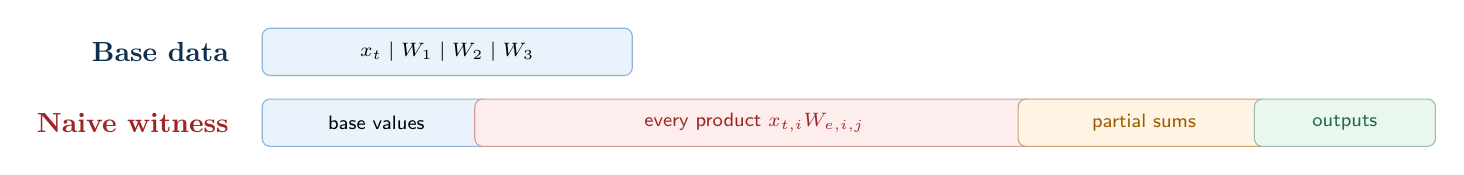
\begin{tikzpicture}[font=\sffamily\scriptsize]
  \node[anchor=east,font=\bfseries\color{navy}] at (0,0.65) {Base data};
  \draw[fill=bluefill,draw=blue!55,rounded corners=1mm] (0.3,.35) rectangle (5.0,.95);
  \node at (2.65,.65) {$x_t\mid W_1\mid W_2\mid W_3$};

  \node[anchor=east,font=\bfseries\color{red}] at (0,-.25) {Naive witness};
  \draw[fill=bluefill,draw=blue!55,rounded corners=1mm] (.3,-.55) rectangle (3.2,.05);
  \node at (1.75,-.25) {base values};
  \draw[fill=redfill,draw=red!45,rounded corners=1mm] (3.0,-.55) rectangle (10.1,.05);
  \node[text=red] at (6.55,-.25) {every product $x_{t,i}W_{e,i,j}$};
  \draw[fill=orangefill,draw=orange!55,rounded corners=1mm] (9.9,-.55) rectangle (13.1,.05);
  \node[text=orange] at (11.5,-.25) {partial sums};
  \draw[fill=greenfill,draw=green!45,rounded corners=1mm] (12.9,-.55) rectangle (15.2,.05);
  \node[text=green] at (14.05,-.25) {outputs};
\end{tikzpicture}

{\sffamily\scriptsize\color{slate}
The commitment itself is not the expansion. The expansion occurs when each operation result is appended to the witness that is committed.}
\end{center}

{\sffamily\bfseries\color{navy}C. Projection compresses the active route}

\begin{center}
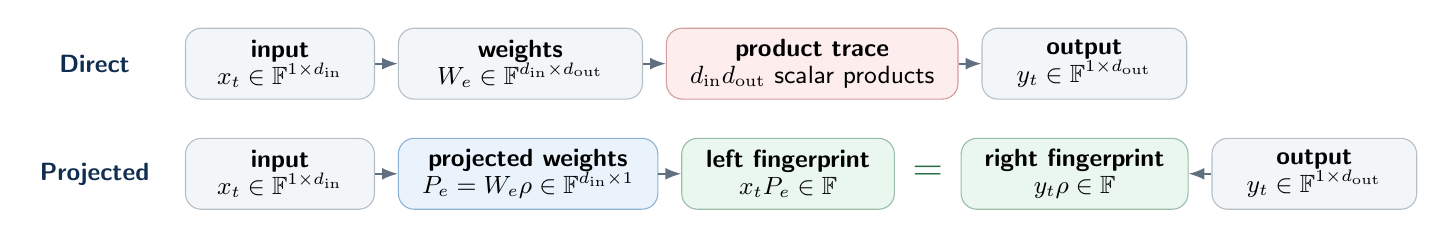
\begin{tikzpicture}[node distance=2.9mm]
  \node[font=\sffamily\bfseries\small\color{navy},minimum width=17mm] (dl) {Direct};
  \node[neutral,minimum width=24mm,right=of dl] (dx) {\textbf{input}\\[-1pt]$x_t\in\mathbb F^{1\times d_{\mathrm{in}}}$};
  \node[neutral,minimum width=31mm,right=of dx] (dw) {\textbf{weights}\\[-1pt]$W_e\in\mathbb F^{d_{\mathrm{in}}\times d_{\mathrm{out}}}$};
  \node[active,minimum width=36mm,right=of dw] (dt) {\textbf{product trace}\\[-1pt]$d_{\mathrm{in}}d_{\mathrm{out}}$ scalar products};
  \node[neutral,minimum width=26mm,right=of dt] (dy) {\textbf{output}\\[-1pt]$y_t\in\mathbb F^{1\times d_{\mathrm{out}}}$};
  \draw[flow] (dx)--(dw); \draw[flow] (dw)--(dt); \draw[flow] (dt)--(dy);

  \node[font=\sffamily\bfseries\small\color{navy},minimum width=17mm,below=9mm of dl] (pjl) {Projected};
  \node[neutral,minimum width=24mm,right=of pjl] (px) {\textbf{input}\\[-1pt]$x_t\in\mathbb F^{1\times d_{\mathrm{in}}}$};
  \node[base,minimum width=32mm,right=of px] (pp) {\textbf{projected weights}\\[-1pt]$P_e=W_e\rho\in\mathbb F^{d_{\mathrm{in}}\times1}$};
  \node[good,minimum width=27mm,right=of pp] (pl) {\textbf{left fingerprint}\\[-1pt]$x_tP_e\in\mathbb F$};
  \node[font=\sffamily\bfseries\Large\color{green},right=1mm of pl] (eq) {$=$};
  \node[good,minimum width=27mm,right=1mm of eq] (pr) {\textbf{right fingerprint}\\[-1pt]$y_t\rho\in\mathbb F$};
  \node[neutral,minimum width=26mm,right=of pr] (py) {\textbf{output}\\[-1pt]$y_t\in\mathbb F^{1\times d_{\mathrm{out}}}$};
  \draw[flow] (px)--(pp); \draw[flow] (pp)--(pl); \draw[flow] (py)--(pr);
\end{tikzpicture}

{\sffamily\scriptsize\color{slate}
The verifier samples $\rho\in\mathbb F^{d_{\mathrm{out}}\times1}$ after commitments. Public-scalar work in $W_e\rho$ is linear; the nonlinear trace falls from $d_{\mathrm{in}}d_{\mathrm{out}}$ to $d_{\mathrm{in}}$ products per route.}
\end{center}

\begin{ideabox}
\textbf{\color{navy}Two distinct savings.} Routing removes computation traces of inactive experts.
Projection then compresses the matrix-multiplication trace of the active expert. Base weights remain
committed, but per-operation products are not appended for inactive routes.
\end{ideabox}

\newpage

\section*{2. Protocol sequence}

\begin{enumerate}
  \item \textbf{\color{navy}Commit first.} The prover fixes the weight matrix $W_e$ and claimed output $y_t$
        before seeing the verifier's randomness.
  \item \textbf{\color{navy}Sample the challenge.} The verifier samples
        $\rho\in\mathbb F^{d_{\mathrm{out}}\times1}$ only after those commitments.
  \item \textbf{\color{navy}Project the weights.} The prover computes
        $P_e=W_e\rho\in\mathbb F^{d_{\mathrm{in}}\times1}$ and proves that $P_e$ was derived from the committed $W_e$.
  \item \textbf{\color{navy}Check one fingerprint.} The verifier checks $y_t\rho=x_tP_e$. If
        $y_t=x_tW_e$, then
        \[
          y_t\rho=(x_tW_e)\rho=x_t(W_e\rho)=x_tP_e.
        \]
\end{enumerate}

\begin{center}
  {\Large\bfseries\color{navy}$\boxed{\;y_t\rho=x_tP_e=x_t(W_e\rho)\;}$}
\end{center}

\section*{3. Numerical example}

Let
\[
X=\begin{pmatrix}2&3\end{pmatrix}\in\mathbb F^{1\times2},
\qquad
W=\begin{pmatrix}1&4&2\\5&0&6\end{pmatrix}\in\mathbb F^{2\times3}.
\]
Ordinary matrix multiplication gives
\[
Y=XW
=\begin{pmatrix}2&3\end{pmatrix}
 \begin{pmatrix}1&4&2\\5&0&6\end{pmatrix}
=\begin{pmatrix}17&8&22\end{pmatrix}
\in\mathbb F^{1\times3}.
\]

After $W$ and $Y$ are fixed, the verifier samples
\[
\rho=\begin{pmatrix}7\\11\\19\end{pmatrix}\in\mathbb F^{3\times1}.
\]
The prover projects the weights:
\[
P=W\rho
=\begin{pmatrix}1&4&2\\5&0&6\end{pmatrix}
 \begin{pmatrix}7\\11\\19\end{pmatrix}
=\begin{pmatrix}89\\149\end{pmatrix}
\in\mathbb F^{2\times1}.
\]
The verifier compares the two scalar fingerprints:
\[
\underbrace{Y\rho}_{\text{output fingerprint}}
=\begin{pmatrix}17&8&22\end{pmatrix}
 \begin{pmatrix}7\\11\\19\end{pmatrix}
=625,
\qquad
\underbrace{XP}_{\text{input/weight fingerprint}}
=\begin{pmatrix}2&3\end{pmatrix}
 \begin{pmatrix}89\\149\end{pmatrix}
=625.
\]

\begin{resultbox}
\textbf{\color{green}Result.} Both fingerprints equal $625$. A false output $Y'$ would pass only if its
nonzero error $\Delta=Y'-XW$ happened to satisfy $\Delta\rho=0$. Because $\rho$ is sampled after
$Y'$ is fixed, this occurs with probability at most about $1/|\mathbb F|$ for a uniform field challenge.
\end{resultbox}

\section*{4. What is actually saved}

The original inference still computes the complete output, and projection adds linear arithmetic.
The saving is inside the proof: a direct active-route trace uses
$\Theta(d_{\mathrm{in}}d_{\mathrm{out}})$ nonlinear multiplication cells, while the projected check uses
$\Theta(d_{\mathrm{in}})$ such cells plus linear work for $W_e\rho$ and $y_t\rho$.
The advantage is substantial for large matrices; for a tiny one-off multiplication, projection may add work rather than save it.

\newpage

\section*{5. Before / after: the cost model in formulas}

\textbf{\color{navy}Baseline.} ``Before'' is the full-witness pipeline this work started from:
expert weights sit in the committed witness and every proved multiplication contributes its own
witness cells. ``After'' is the routed-projected protocol of
\texttt{analysis/routed-projected-protocol.md}. Both sides are priced with the same Ligero cost
structure and the same code base; no unrelated optimization enters either side of the comparison.

{\sffamily\bfseries\color{navy}A. One routed matmul, per token}

For $X_t\in\mathbb F^{1\times K}$, $W_e\in\mathbb F^{K\times J}$
($K=d_{\mathrm{in}}$, $J=d_{\mathrm{out}}$), the per-token cell counts are
\[
\underbrace{w_{\mathrm{dir}}=KJ+J}_{\text{products}+\text{outputs}},\qquad
q_{\mathrm{dir}}=KJ
\qquad\Longrightarrow\qquad
\underbrace{w_{\mathrm{proj}}=2K+1}_{H,\;Q,\;y^\rho},\qquad
q_{\mathrm{proj}}=K,
\]
plus, once per expert and amortized over all tokens routed anywhere, $K$ cells for the projected
column $P_e=W_e\rho$, bound by a \emph{public-coefficient linear} relation (no quadratic cells).
The compression factors are
\[
\frac{w_{\mathrm{dir}}}{w_{\mathrm{proj}}}=\frac{KJ+J}{2K+1}\approx\frac{J}{2},
\qquad
\frac{q_{\mathrm{dir}}}{q_{\mathrm{proj}}}=J .
\]
Route hiding changes the two sides asymmetrically: before, hiding $e_t$ forces materializing all
$E$ expert traces ($\times E$ on the dominant term); after, the single matrix $P$ already covers
all $E$ experts at $EK$ cells per layer, so hiding costs $\times E$ only on the projected weights,
never on the traces.

{\sffamily\bfseries\color{navy}B. Full model (Maverick), $S=1000$ tokens}

With $L=24$ MoE layers, $E=128$ experts, $d=5120$, $f=8192$, and three expert matrices per layer
whose contraction dimensions sum to $\sum_m K_m=2d+f$ ($m$ ranges over the $3L=72$ routed matmuls):
\[
N=L\,S\,(2d+f)=442{,}368{,}000,
\qquad
R=L\,E\,(2d+f)=56{,}623{,}104 .
\]
The routed-projected MoE block then costs, row-exactly (ELL $=8192$; the $72$ $y^\rho$ variables
and late Freivalds auxiliaries carry their own padding),
\[
W_{\mathrm{route}}=2N+R+4\cdot72\cdot\mathrm{ELL}=943{,}718{,}400,
\]
\[
L_{\mathrm{route}}=R+2\cdot72\,S+72\,(2E+1)=56{,}785{,}608,
\qquad
Q_{\mathrm{route}}=N+72E=442{,}377{,}216 .
\]
Substituting this block for the ordinary weight-witness block and the $E$ per-expert output
streams gives the whole-proof ledgers (exact values printed by
\texttt{analysis/routed\_projected\_4h\_model.py}):

\begin{center}
\sffamily\small
\begin{tabular}{lrrrr}
\textbf{\color{navy}Ledger} & \textbf{\color{navy}Before} & \textbf{\color{navy}After} & \textbf{\color{navy}Ratio} & \textbf{\color{navy}Speedup}\\[1pt]
\hline\\[-8pt]
Witness cells $W$    & $888{,}249{,}981{,}888$ & $95{,}205{,}646{,}976$ & $10.72\%$ & $\times9.33$\\
Linear cells $L$     & $162{,}237{,}276{,}010$ & $31{,}064{,}630{,}194$ & $19.15\%$ & $\times5.22$\\
Quadratic cells $Q$  & $173{,}106{,}423{,}296$ & $42{,}394{,}577{,}408$ & $24.49\%$ & $\times4.08$\\
\end{tabular}
\end{center}

{\sffamily\bfseries\color{navy}C. From cells to time}

Every prover stage — witness regeneration, encoding, Merkle hashing, the linear/quadratic folds,
column opening — is linear in the cells it touches, so the prove time decomposes as
\[
t_{\mathrm{prove}}
=\sum_{\text{stage }i} c_i\,n_i(W,L,Q),
\qquad
\frac{t^{\mathrm{before}}_i}{t^{\mathrm{after}}_i}
=\frac{n_i(W,L,Q)^{\mathrm{before}}}{n_i(W,L,Q)^{\mathrm{after}}},
\]
with per-kernel constants $c_i$ measured, never fitted globally. Witness-bound stages therefore
speed up by $\times9.33$, linear folds by $\times5.22$, quadratic folds by $\times4.08$. Under the
per-kernel admission model the after-pipeline sums to
\[
t_{\mathrm{prove}}\le 13{,}046.264\ \mathrm{s}=3.6240\ \mathrm{h}
\]
at $S=1000$, inside the four-hour envelope; the before-pipeline is dominated by committing,
encoding and folding the $888$G-cell witness and admits no such envelope on the same hardware.
The soundness price of the entire transformation is
\[
\epsilon_{\mathrm{new}}\le\epsilon_{\mathrm{Ligero}}+\frac{3}{|\mathbb F|}+\epsilon_{\mathrm{hash}} .
\]

\begin{resultbox}
\textbf{\color{green}Before/after in one line.} The projection shrinks the witness $\times9.33$,
the linear ledger $\times5.22$ and the quadratic ledger $\times4.08$ at a soundness cost of
$3/|\mathbb F|$ — an order-of-magnitude smaller proof workload bought with a negligible
field-soundness term.
\end{resultbox}

\end{document}
